\chapter{Dataflow Modeling} \label{ch:dataflowModeling}
\chapterquote{All action results from thought, so it is thoughts that matter.}{Sai Baba}

\graphicspath{{Chapters/Dataflow/Figures/}}
\lstinputpath{Codes-VHDL/Chapter-Dataflow/VHDLCodes} %path is defined in mypreamble


%\section{Introduction}
In this chapter, UART communication is discussed for NIOS design. Values of Sin(x) is generated using NIOS and the data is  received by computer using UART cable. Since, onchip memory is smaller for storing these values, therefore external memory i.e. SDRAM is used. Further, the received data is stored in a file using `Tera Term' software; finally live-plotting of data is performed using Python.  

In this chapter, we will learn following topics, 
\begin{enumerate}
	\item UART interface,
	\item Receiving the data on computer using UART communication,
	\item SDRAM interface,
	\item Saving data generated by NIOS desgin to a file using `Tera Term',
	\item Updating a existing QSys design and corresponding VHDL and NIOS design,
	\item Live-plotting of data using Python. 
\end{enumerate}

\section{UART interface}
First, create a empty project with name `UartComm' (see Section \ref{sec:new_project}). Next, open the QSys from Tools$\rightarrow$Qsys. Add `Nios Processor', `On-chip RAM (with 20k total-memory-size), `JTAG UART' and `UART (RS-232 Serial Port)' (\textbf{all with default settings}). Note that, Baud rate for UART is set to `115200' (see Fig. \ref{fig:uart_settings}), which will be used while getting the data on computer. Lastly, connect these items as shown in Fig. \ref{fig:uart_qsys_conn}; save it as `Uart\_Qsys.qsys' and finally generate the Qsys system and close the Qsys. Please see Section \ref{sec:CreateGenerateQsys}, if you have problem in generating the QSys system.

\begin{figure}[!h]
	\centering
	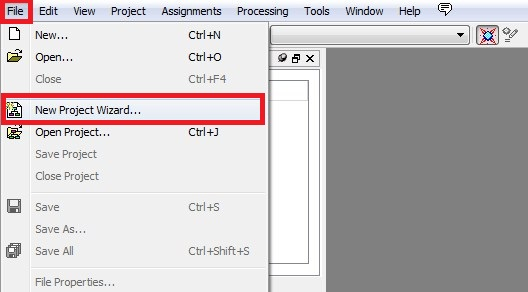
\includegraphics[scale=0.7]{1}
	\caption{UART settings}
	\label{fig:uart_settings}
\end{figure}
 
\begin{figure}[!h]
	\centering
	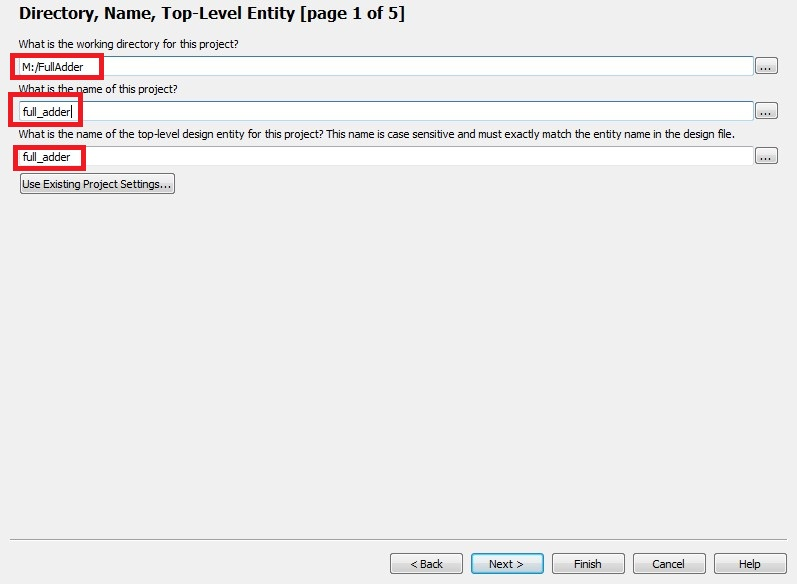
\includegraphics[scale=0.65]{2}
	\caption{Qsys connections}
	\label{fig:uart_qsys_conn}
\end{figure}

Now, add the file `Uart\_Qsys.qip' to the VHDL project. Next, create a new `Block diagram (.bdf) file and import the Qsys design to it and assign correct pin numbers to it, as shown in Fig. \ref{fig:uart_top}. Save it as `Uart\_top.bdf' and set it as `top  level entity'. Lastly, import the pin assignment file and compile the design. Finally, load the design on FPGA board. 

\begin{figure}[!h]
	\centering
	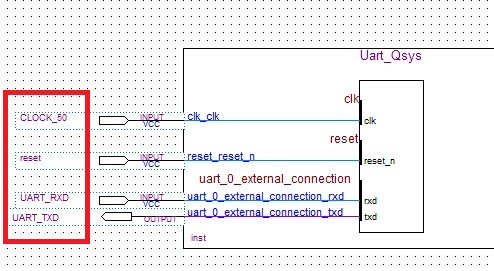
\includegraphics[scale=0.65]{3}
	\caption{Top level entity `Uart\_top.bdf'}
	\label{fig:uart_top}
\end{figure}

\section{NIOS design}
In Chapter \ref{ch:NiosOverview}, we created the `BSP' and `application' file separately for NIOS design. In this chapter, we will use the template provided with NIOS to create the design. For this, open the NIOS software and go to `Files$\rightarrow$New$\rightarrow$NIOS II Application and BSP from Template'. Next, Select the `UART\_Qsys.sopcinfo' file and `Hello World' template and provide the desired name to project e.g. UART\_comm\_app, as shown in Fig , and click `next'. In this window, enter the desired name for BSP file in the `Project name' column e.g. `UART\_comm\_bsp'; and click on Finish.  

\begin{figure}[!h]
	\centering
	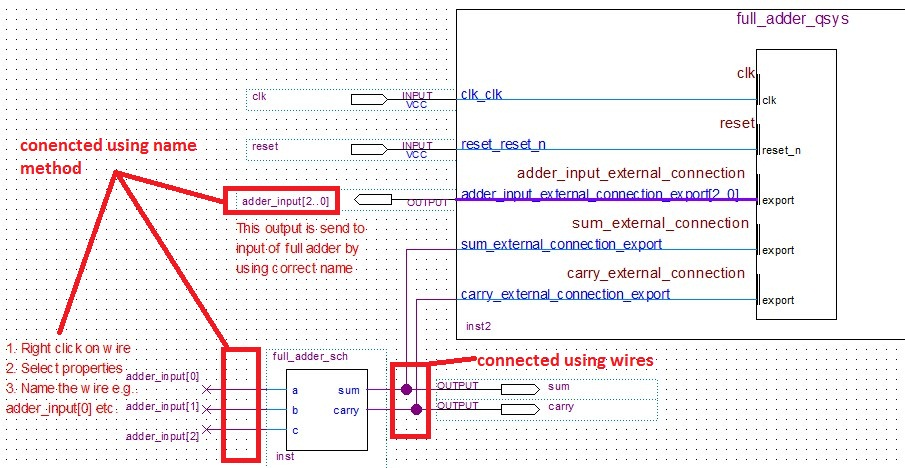
\includegraphics[scale=0.65]{4}
	\caption{Create NIOS project from template}
	\label{fig:nios_name_uart}
\end{figure}

\section{Communication through UART}
To received the data on computer, we need some software like Putty or Tera Term. In this tutorial, we are using `Tera Term software, which can be downloaded freely. Also, we need to change the UART communication settings; so that, we can get messages through UART interface (instead of JTAG-UART)  as shown next. 

Right click on `UART\_comm\_bsp' and go to `NIOS II$\rightarrow$BSP editor'; and select UART\_115200 for various communication as shown in Fig \ref{fig:nios_uart_settings}; and finally click on generate and then click on exit. Now, all the 	`printf' statements will be send to computer via UART port (instead of Jtag-uart). We can change it to JTAG-UART again, by changing UART\_115200 to JTAG-UART again. Note that, when we modify the BSP using BSP-editor, then we need to generate the system again.

\begin{figure}[!h]
	\centering
	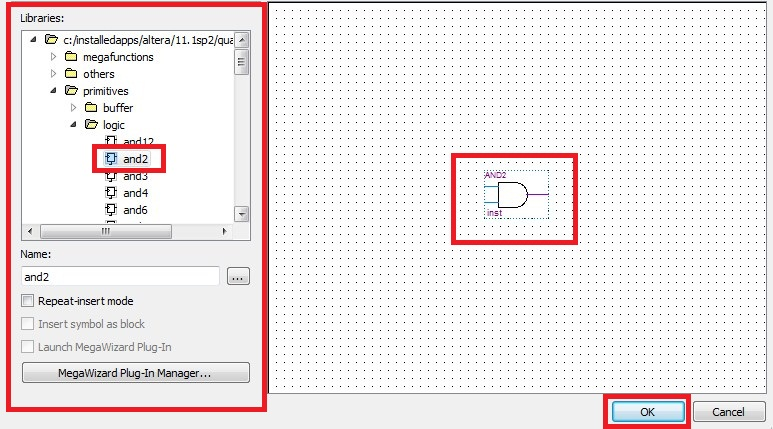
\includegraphics[scale=0.65]{5}
	\caption{UART communication settings in NIOS}
	\label{fig:nios_uart_settings}
\end{figure}

Now, open the Tera Term and select the `Serial' as shown in Fig. \ref{fig:teraTerm}. Then go to `Setup$\rightarrow$Serial Port...' and select the correct baud rate i.e. 115200 and click OK, as shown in Fig. \ref{fig:baudRateteraTerm}. 

\begin{figure}[!h]
	\centering
	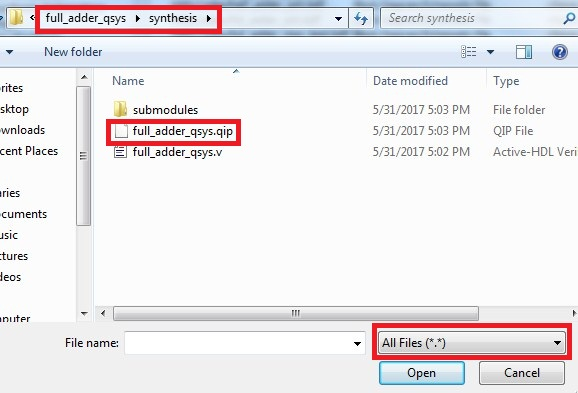
\includegraphics[scale=0.65]{6}
	\caption{Serial communication in Tera Term}
	\label{fig:teraTerm}
\end{figure}

\begin{figure}[!h]
	\centering
	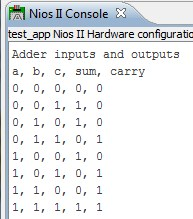
\includegraphics[scale=0.65]{7}
	\caption{Select correct baud rate}
	\label{fig:baudRateteraTerm}
\end{figure}

Finally, right click on `UART\_comm\_app' in NIOS and go to `Run As$\rightarrow$3 NIOS 2 Hardware'. Now, we can see the output on the Tera Term terminal, as shown in Fig. \ref{fig:helloTera}. 

\begin{figure}[!h]
	\centering
	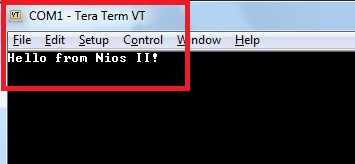
\includegraphics[scale=0.65]{8}
	\caption{`Hello from NIOS II!' on Tera Term}
	\label{fig:helloTera}
\end{figure}

\section{SDRAM Interface}
Our next aim is to generate the Sine waves using NIOS and then plot the waveforms using python. If we write the C-code in current design, then our system will report the memory issue as onchip memory is too small; therefore we need to use external memory. In this section, first, we will update the Qsys design with SDRAM interface, then we will update the Quartus design and finally add the C-code to generate the Sine waves. 

\subsection{Modify QSys}
First, Open the UART\_Qsys.qsys file in QSys software. Now, add SDRAM controller with default settings,  as shown in Fig. \ref{fig:sdram_con}. Next, connect all the ports of SDRMA as shown in Fig. \ref{fig:sdram_connections}. Then, double click the `nios2\_qsys\_0' and select `SDRAM' as reset and exception vector memory, as shown in Fig. \ref{fig:sdram_vector_memory}. 

\begin{figure}[!h]
	\centering
	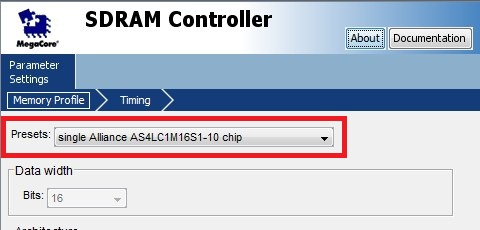
\includegraphics[scale=0.6]{9}
	\caption{SDRAM controller}
	\label{fig:sdram_con}
\end{figure}


\begin{figure}[!h]
	\centering
	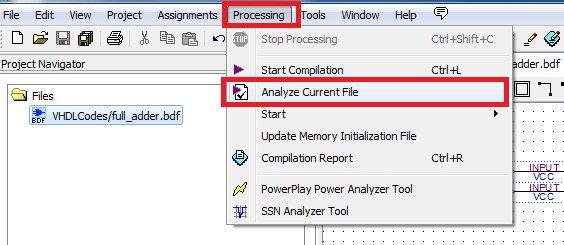
\includegraphics[scale=0.6]{10}
	\caption{SDRAM connections}
	\label{fig:sdram_connections}
\end{figure}


\begin{figure}[!h]
	\centering
	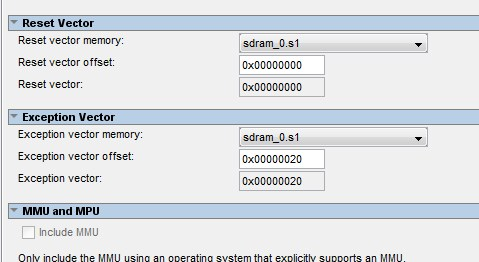
\includegraphics[scale=0.6]{11}
	\caption{Select SDRAM as vector memories}
	\label{fig:sdram_vector_memory}
\end{figure}


Next, we will add `Switches' to control the amplitude of the sine waves. For this add the PIO device of `8 bit with type input', and rename it as `switch', as shown in Fig. \ref{fig:switchForAmplitude} . Finally, go to System$\rightarrow$Assign base addresses, and generate the system. 

\begin{figure}[!h]
	\centering
	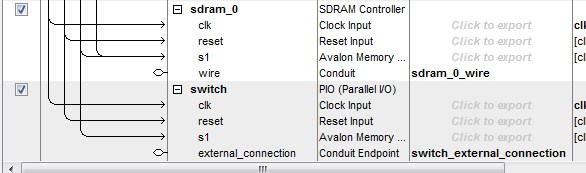
\includegraphics[scale=0.65]{12}
	\caption{Add switches for controlling the amplitude of sine waves}
	\label{fig:switchForAmplitude}
\end{figure}


\subsection{Modify Top level Quartus design}
Now, open the `Uart\_top.bdf' file in Quartus. Right click on the `Uart\_Qsys' block and select `Update symbol or block'; then select the option `Selected symbol(s) or block(s)' and press OK. It will display all the ports for `SDRAM' and switches. Next, we need to assign the correct `pin names' to these ports, as shown in Fig. \ref{fig:SDRAM_Pinassg}.  

\begin{figure}[!h]
	\centering
	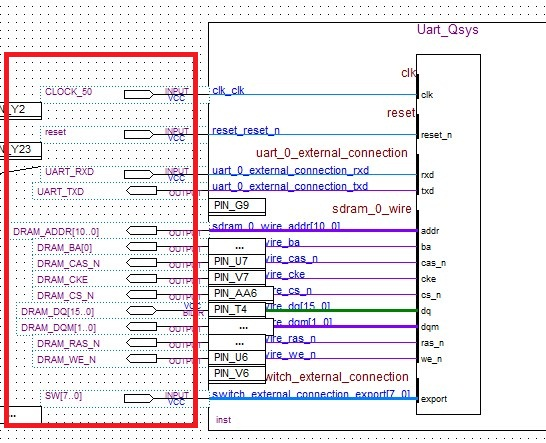
\includegraphics[scale=0.65]{13}
	\caption{Assigning Pins to SDRAM and Switches}
	\label{fig:SDRAM_Pinassg}
\end{figure}

Note that, there should be `-3 ns clock delay' for SDRAM as compare to FPGA clock, therefore we need to add the clock with `-3 ns delay'. For this, double click on the Uart\_top.bdf (anywhere in the file), and select `MegaWizard Plug-In Manager'. Then select `Create a new custom megafunction variation' in the popped-up window and click next. Now, select \textbf{ALTPLL} from \textbf{IO} in \textbf{Installed Plug-Ins} option, as shown in Fig. \ref{fig:dram_clock_altpll}, and click next. Then, follow the figures from Fig. \ref{fig:altpllCreation1} to Fig. \ref{fig:altpllCreation6} to add the ALTPLL to current design i.e. `Uart\_top.bdf'. Finally, connect the ports of this design as shown in Fig. \ref{fig:altpllCreation7}. Note that, in these connections, output of ATLPLL design is connected to `DRAM\_CLK', which is clock-port for DRAM. Lastly, compile and load the design on FPGA board. 

\begin{figure}[!h]
	\centering
	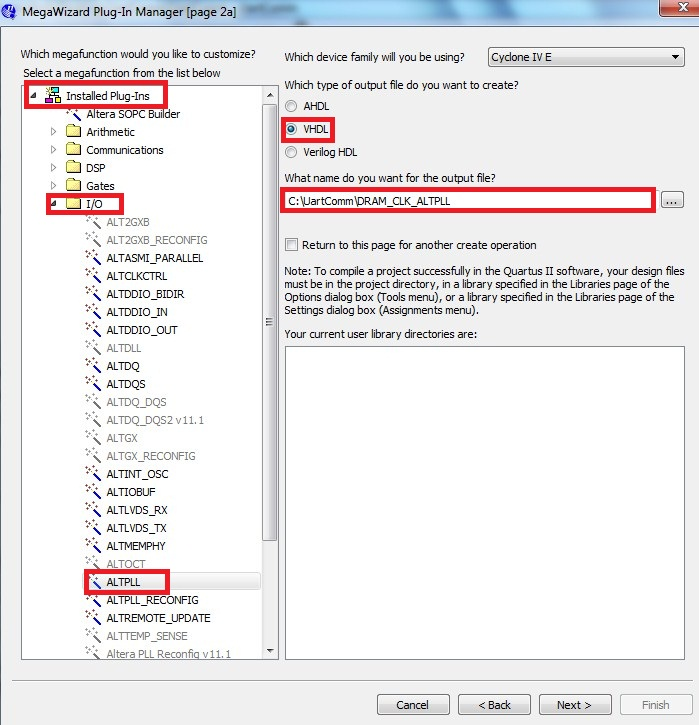
\includegraphics[scale=0.4]{14}
	\caption{ALTPLL generation}
	\label{fig:dram_clock_altpll}
\end{figure}

\begin{figure}[!h]
	\centering
	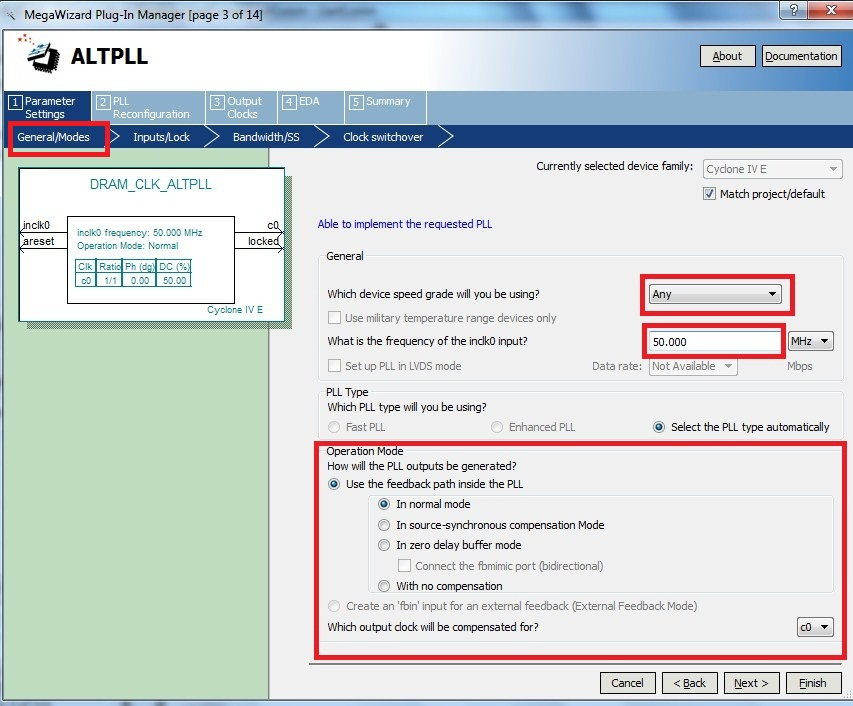
\includegraphics[scale=0.4]{15}
	\caption{ALTPLL creation, step 1}
	\label{fig:altpllCreation1}
\end{figure}

\begin{figure}[!h]
	\centering
	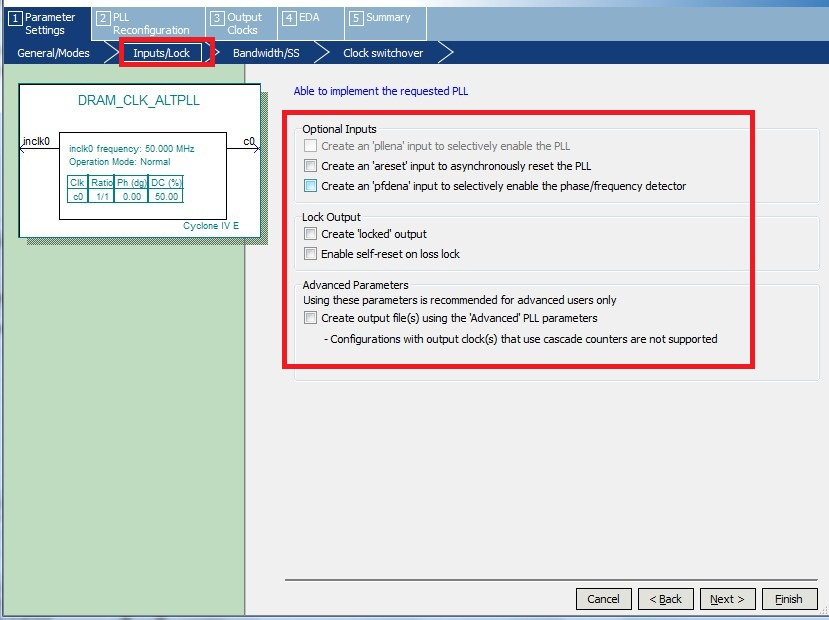
\includegraphics[scale=0.5]{16}
	\caption{ALTPLL creation, step 2}
	\label{fig:altpllCreation2}
\end{figure}

\begin{figure}[!h]
	\centering
	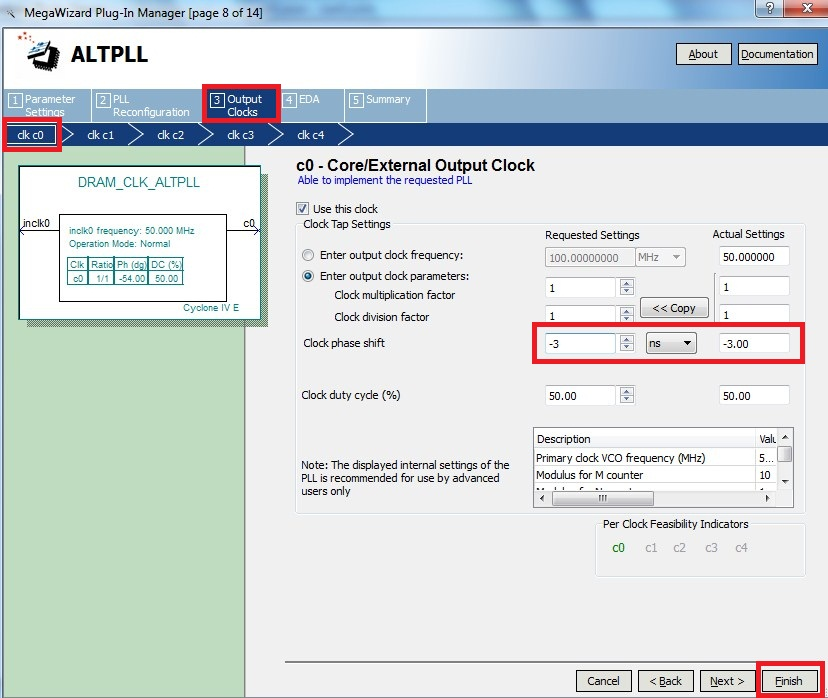
\includegraphics[scale=0.4]{17}
	\caption{ALTPLL creation, step 3}
	\label{fig:altpllCreation3}
\end{figure}

\begin{figure}[!h]
	\centering
	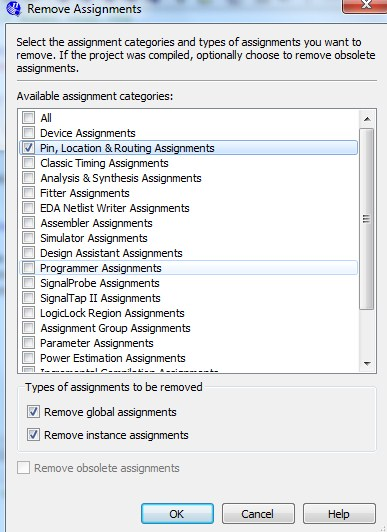
\includegraphics[scale=0.4]{18}
	\caption{ALTPLL creation, step 4}
	\label{fig:altpllCreation4}
\end{figure}

\begin{figure}[!h]
	\centering
	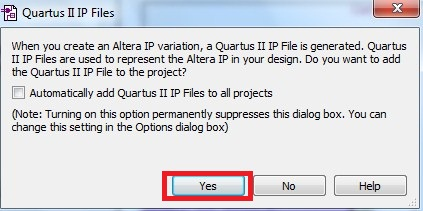
\includegraphics[scale=0.5]{19}
	\caption{ALTPLL creation, step 5}
	\label{fig:altpllCreation5}
\end{figure}

\begin{figure}[!h]
	\centering
	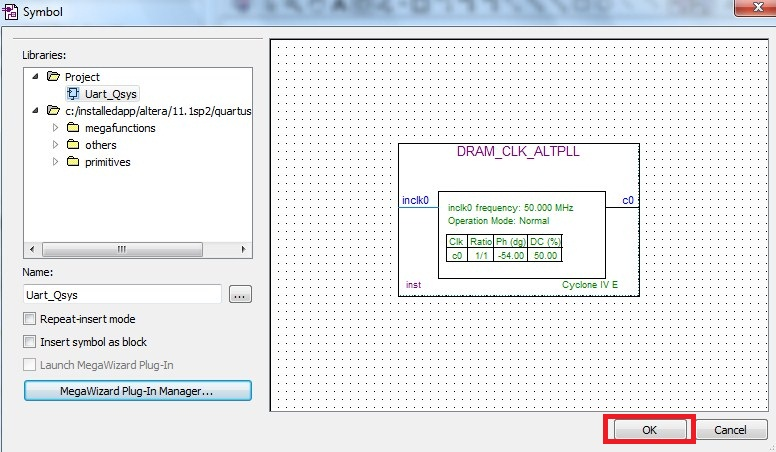
\includegraphics[scale=0.5]{20}
	\caption{ALTPLL creation, step 6}
	\label{fig:altpllCreation6}
\end{figure}

\begin{figure}[!h]
	\centering
	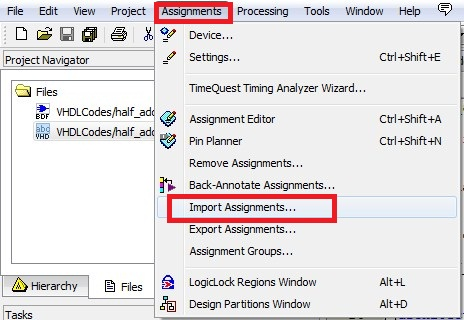
\includegraphics[scale=0.6]{21}
	\caption{Connect ALTPLL design with existing design}
	\label{fig:altpllCreation7}
\end{figure}

\subsection{Updating NIOS design}
Since, we have udpated the QSys design, therefore the corresponding .sopcinfo file is also updated. Further, BSP files depends on the .sopcinfo file, therefore we need to update the BSP as well. For this, right click on `Uart\_comm\_bsp' and go to `NIOS II$\rightarrow$BSP Editor; and update the BSP as shown in Fig. \ref{fig:updateBSPDRAM} and click on `generate' and then click `exit'. Note that, `enable' options are unchecked now, because we are using External memory, which is quite bigger than onchip-memory, so we do not need `small' size options. 

\begin{figure}[!h]
	\centering
	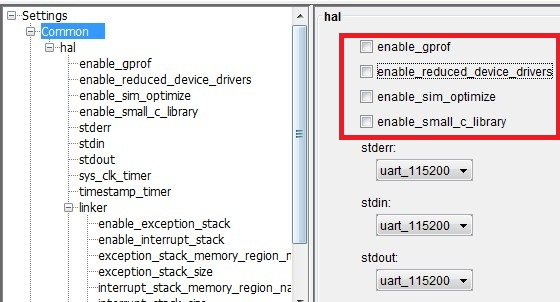
\includegraphics[scale=0.65]{22}
	\caption{Update BSP for new Qsys design}
	\label{fig:updateBSPDRAM}
\end{figure}

Now, update the `hello\_world.c' file as shown in Listing \ref{c:uart_sine_wave}. 

\lstinputlisting[
caption    = {Sin and Cos wave generation},
language = C,
label      = {c:uart_sine_wave}
]{CppCodes/hello_world.c}

In Tera Term, we can save the received values in text file as well. Next, go Files$\rightarrow$Log and select the filename at desired location to save the data e.g. `sineData.txt'. 

Finally, right click on `UART\_comm\_app' in NIOS and go to `Run As$\rightarrow$3 NIOS 2 Hardware'. Now, we can see the decimal values on the screen. If all the switches are at `0' position, then values will be `0.000' as amplitude is zero. Further, we can use any combination of 8 Switches to increase the amplitude of the sine and cosine waves. Also, result will be stored in the  `sineData.txt' file. Content of this file is shown in Fig. \ref{fig:contentLogFile}


\begin{figure}[!h]
	\centering
	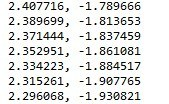
\includegraphics[scale=0.8]{23}
	\caption{Content of `sineData.txt' file}
	\label{fig:contentLogFile}
\end{figure}

\section{Live plotting the data}
In the previous section, we store the sine and cosine wave data on the `sineData.txt' using UART communication. Now, our last task is to plot this data continuously, so that it look line animation. For this save the Listing \ref{pythhon:plotLogData}, in the location where `sineData.txt' is saved. Now, open the command prompt and go to the location of python file. Finally, type \textbf{`python main.py'} and press enter. This will start plotting the waveform continuously based on the data received and stored on the `sineData.txt' file. The corresponding plots are shown in Fig. \ref{fig:plotLogFile}.

\lstinputlisting[
caption    = {Code for live plotting of logged data},
language = Python,
label      = {pythhon:plotLogData}
]{PythonCodes/main.py}

\begin{figure}[!h]
	\centering
	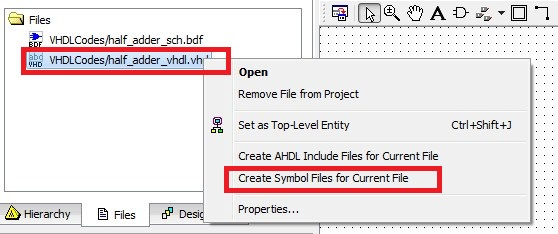
\includegraphics[scale=0.5]{24}
	\caption{Plot of `sineData.txt' file}
	\label{fig:plotLogFile}
\end{figure}


\section{Conclusion}
In this chapter, first we display the `Hello' message using UART and Tera Term. Then, SDRAM is included in the design and correspondingly all the other designs are updated i.e. Quartus and NIOS. Then, the data is stored in the text file and finally it is plotted with the help of Python programming language. 

\section{Introduction}
In Chapter \ref{ch:OverView} and \ref{ch:Datatypes}, we saw various elements of VHDL language along with several examples. More specifically, Chapter \ref{ch:OverView} presented various ways to design the `comparator circuits' i.e. using dataflow modeling, structural modeling and packages etc.; and then Chapter \ref{ch:Datatypes} presented various elements of VHDL language which can be used to implement the digital designs. These two chapters are the foundation of the VHDL language, and the illustrated designs-examples were not of any particular usage (especially in Chapter \ref{ch:Datatypes}). From this chapter we will concentrate on the proper digital design using various elements of VHDL which are described in previous chapters.  

In this chapter, differences between `combinational designs' and `sequential designs' are shown. Also, various methods are discussed which are used for designing the `combinational circuit' and `sequential circuits'. Main focus of this chapter is the `combinational designs' using `Dataflow' modeling style; in which functionality of the entity is described using `concurrent statements' (without defining the structure of the design); whereas Chapter \ref{ch:behavioralModeling} will present the `behavioral modeling' which can be used to create both `sequential' and `combinational' design. 

\section{Combinational circuit and sequential circuit}\label{sec:combSeqCircuit}\index{combination circuit}\index{sequential circuit}

Digital design can be broadly categorize in two ways i.e. \textbf{combinational designs} and \textbf{sequential designs}. It is very important to understand the difference between these two designs and see the relation between these designs with various elements of VHDL. 
\begin{enumerate}
	\item \textbf{Combinational designs} : Combinational designs are the designs in which output of the system depends on present value of the inputs only. Since, the outputs depends on current inputs only, therefore `\textbf{no memory}' is required for these designs. Further, memories are nothing but the `flip flops' in the digital designs, therefore there is \textbf{no need of `flip flops'} in combination designs. In the other words, only `logic gates (i.e. and, not and xor etc.)' are required to implement the combinational designs.
	
	\item \textbf{Sequential designs} : Sequential designs are the designs in which the output depends on current inputs and previous states of the system. Since output depends on previous states, therefore `\textbf{memories}' are required for these systems. Hence, in sequential designs the `flip flops' are need along with the logic gates. 
\end{enumerate}

\begin{noNumBox}
	Remember : 
	\begin{enumerate}
		\item Only `logic gates (i.e. and, not and xor etc.)' are required to implement the combinational designs.
		\item Both `logic gates' and `flip flops' are required for implementing the sequential designs. 
		\item Lastly, the `sequential design' contains both `combinational logic' and `sequential logic', but the combinational logic can be implement using `sequential statements' only as shown in Fig. \ref{fig:combSeqBlock}; whereas the `combination logic' can be implement using `concurrent or sequential statement' in the combinational designs. These statements are discussed in Section \ref{sec:concurrentSeq}. 
	\end{enumerate}
\end{noNumBox}

\begin{figure}[!h]
	\centering
	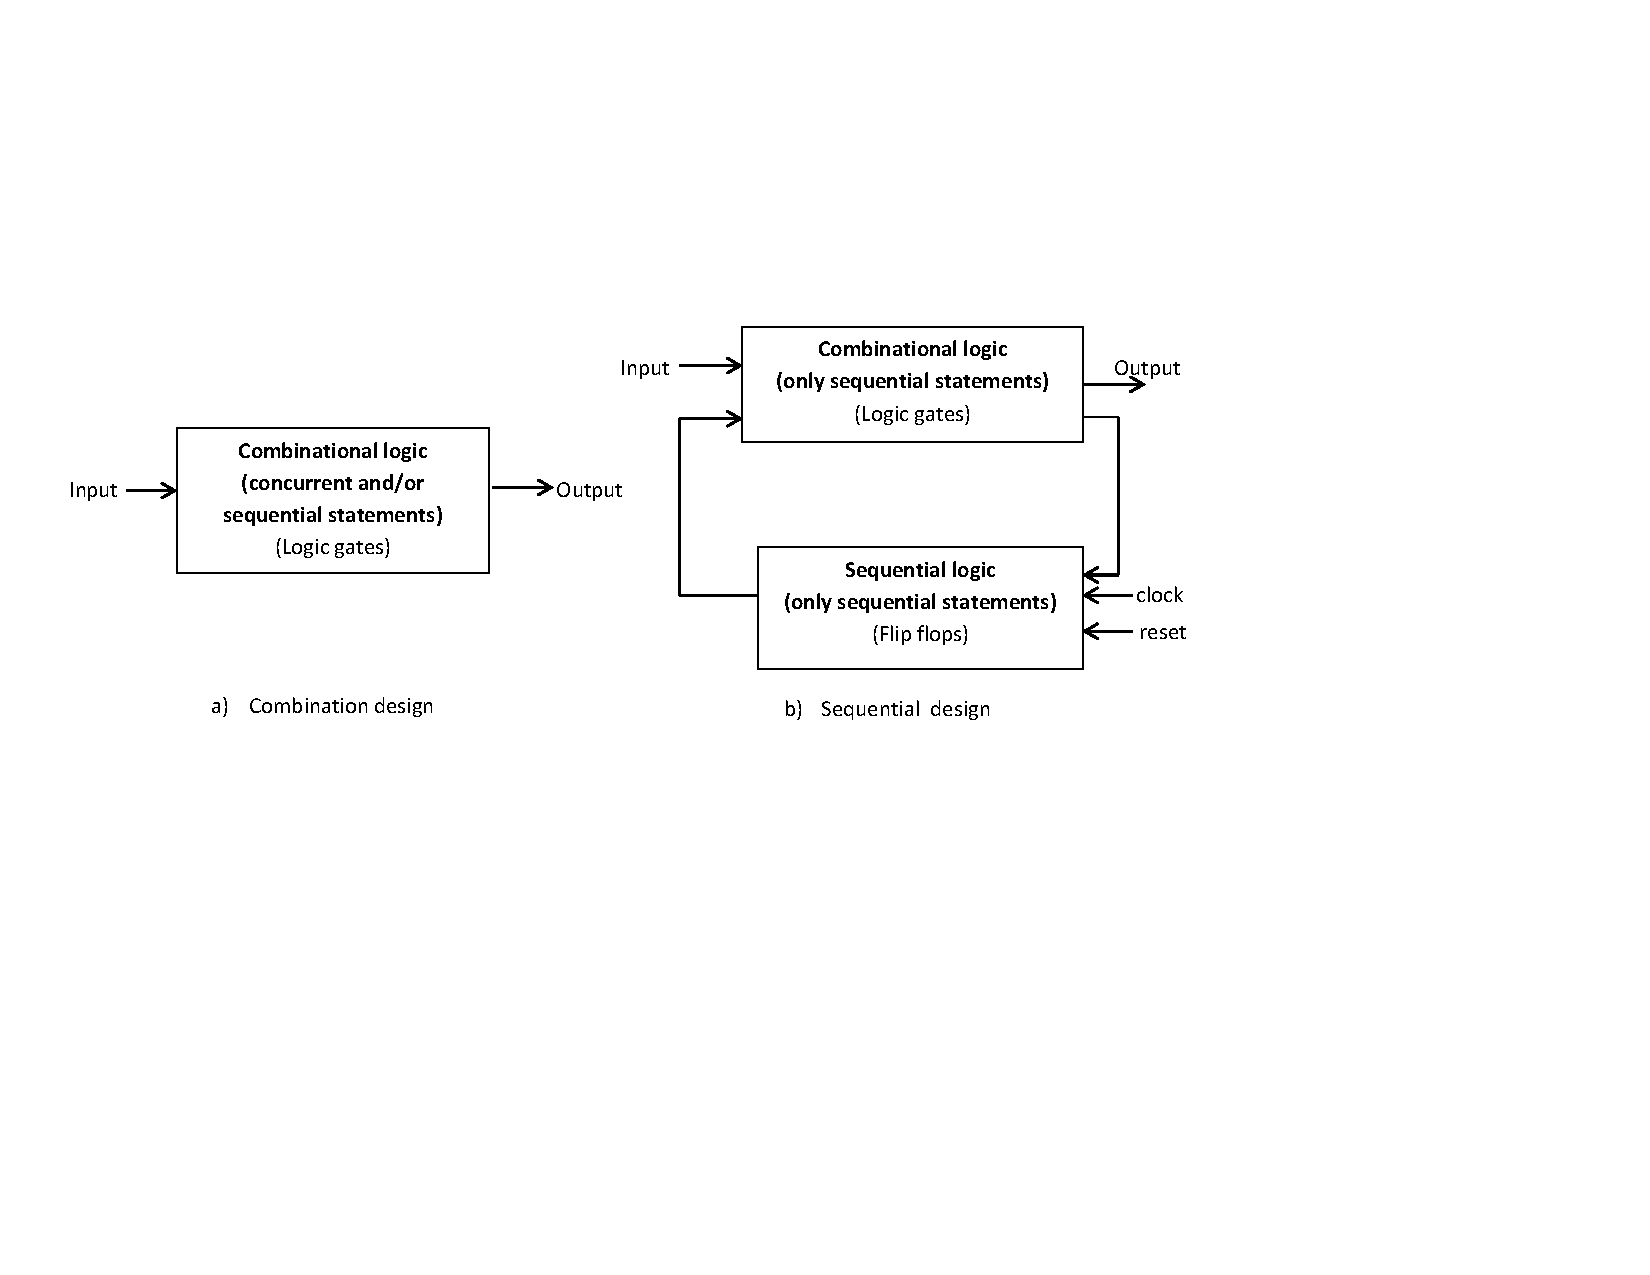
\includegraphics[scale=0.8]{combSeqBlock}
	\caption{Block diagram of `combinational' and `sequential' designs}
	\label{fig:combSeqBlock}
\end{figure}


\section{Concurrent statements and sequential statements}\label{sec:concurrentSeq}

In Section \ref{sec:dataflowOverview}, we saw that the concurrent statements execute in parallel, i.e. the order of the statement does not matter. Whereas in Section \ref{sec:behaviourModeling} shows the example of `sequential statements' where the statements execute one by one. Following are the relationship between `statements' and `design-type', which are illustrated in Table \ref{tbl:CombSeq} as well. 

\begin{enumerate}
	\item Please note that `sequential statements' and `sequential designs' are two different things. Do not mix these together.
	\item Combinational designs can be implemented using both `sequential statements' and `concurrent statements'. 
	\item Sequential designs can be implemented using `sequential statements' only. 
	\item Sequential statements can be defined inside `process' , `function' and `procedure' block only. Further, these blocks executes concurrently e.g. if we have more than one process block then these block will execute in parallel, but statements inside each block will execute sequentially. 
	\item VHDL constructs for combinational designs are `when-else', `with-select' and `generate', which are discussed in this chapter. 
	\item VHDL constructs for sequential designs are `if', `loop', `case' and `wait', which are discussed in Chapter \ref{ch:behavioralModeling}.
\end{enumerate}

\begin{table}[!h]
	\centering
	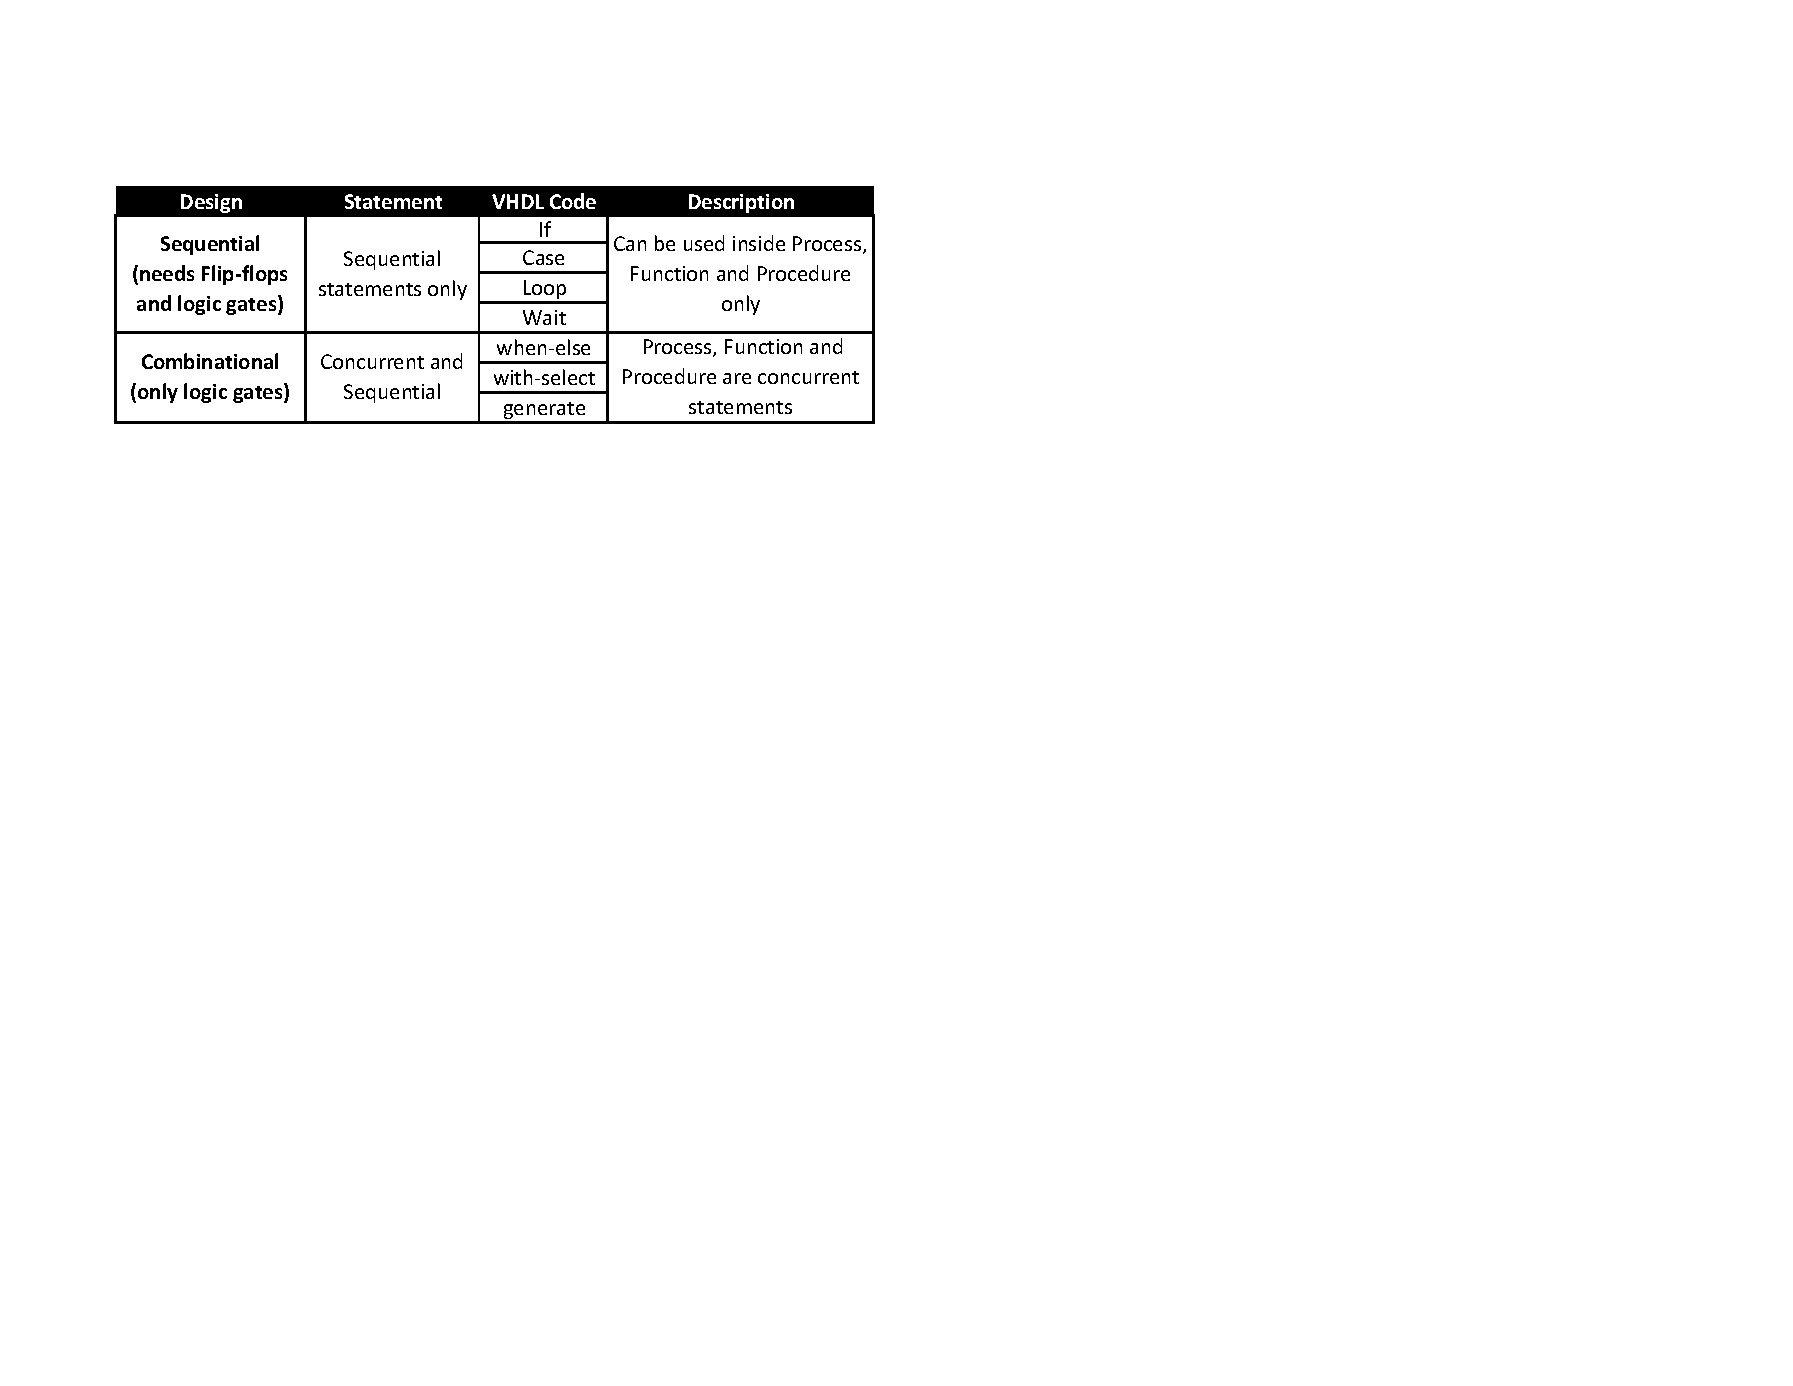
\includegraphics[scale = 0.9]{CombSeq}
	\caption{Relationship between `design-type' and `statements'}
	\label{tbl:CombSeq}
\end{table}

\section{Delay in signal assignments}
In Chapter \ref{ch:OverView}, we saw that concurrent statements do not execute sequentially i.e. order of statements do not matter in concurrent statements. More precisely, these statements are `event triggered' statements i.e. these statements execute whenever there is any event on the signal, as discussed in Listing \ref{vhdl:deltaDelayEx} and \ref{vhdl:afterDelay}.

Remember that, lines 15 and 16 in Listing \ref{vhdl:deltaDelayEx} and \ref{vhdl:afterDelay} are the example of signal assignments. In this section, two types of delays in signal assignments, i.e. `delta delay ($\Delta t$)' and `delay using `after' statement', are discussed. 

\subsection{Delta delay}
If `no delay' or delay of `0 ns' is specified in the statement, then delta delay is assumed in the design. These two delays are shown in Listing \ref{vhdl:deltaDelayEx} which is explain below. 
\begin{explanation}[Listing \ref{vhdl:deltaDelayEx}]
	In this listing, `x' and `z' are the input and output ports respectively, whereas `s' is the signal. In line 15, delay is not defined explicitly; whereas in Line 16, 0 ns delay is defined. Hence, in both the cases `delta delay ($\Delta t$)' is assumed which is explained in next paragraph. 
	
	As explained before, concurrent statements execute whenever there is any change in the signals; therefore line 16 will be executed, when there is any change in the input `x'. This statement will execute in $\Delta t$ time. Hence, the value of signals `s' will be changed after $\Delta t$ time. Since the value of `s' is changed, therefore in next $\Delta t$ time, line 15 will execute and the value of `z' will be changed. 
	
	In the other words, the code will execute `two times' in $2\Delta t$ time to complete the signal assignments; in first $\Delta t$ time, value of `s' will change and in next $\Delta t$ time, the value of `s' will be assigned to `z'. In general, code will execute until there is no further change in the signals. Also, delta delay is very small and can not be seen in simulation results as illustrated in Fig. \ref  {fig:deltaDelayEx}.	Further, in the figure, all the values i.e. `x', `s' and `z' are changed at the same time, which indicates that delta delay is very small and can not be observed. 
	
	\begin{noNumBox}
		Note that	multiple signal assignments are not allowed in VHDL, as shown in line 17 of Listing \ref{vhdl:deltaDelayEx}. Here, signal assignment for `z' is done twice i.e. line 15 and 17. If we uncomment the line 17, then model will be invalid and error will be generated. 
	\end{noNumBox}
\end{explanation}

\lstinputlisting[
language = Vhdl,
caption    = {Delta delay},
label      = {vhdl:deltaDelayEx}
]{deltaDelayEx.vhd}

\begin{figure}[!h]
	\centering
	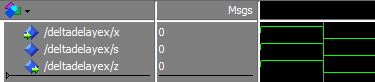
\includegraphics{deltaDelayEx}
	\caption{Delta delay}
	\label{fig:deltaDelayEx}
\end{figure}

\subsection{Delay with `after' statement}
We can assign the desired delay in the signal assignment statement as shown in lines 15 and 16 of Listing \ref{vhdl:afterDelay}. Here signal `s' is assigned after the delayed of 1 ns (line 15), then the value of `s' is assign to `z' after 1 ns (line 16). Hence the output `z' will be delay by 2 ns with respect to `x' as shown in Fig. \ref{fig:afterDelay} using vertical red lines (which show the propagation of value `1'). Also, horizontal red lines for `s' and `z' show that these signals are uninitialized for that time period (because values are assigned after 1 and 2 ns respectively). 


\lstinputlisting[
language = Vhdl,
caption    = {Specify delay using `after'},
label      = {vhdl:afterDelay}
]{afterDelay.vhd}

\begin{figure}[!h]
	\centering
	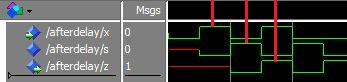
\includegraphics{afterDelay}
	\caption{Delay}
	\label{fig:afterDelay}
\end{figure}

\section{Concurrent signal assignments}
Similar to `if' statement in behavioral modeling, the `dataflow' modeling provides two signal assignments i.e. `Conditional signal assignment' and `Selected signal assignment'. In this chapter, the multiplexer is designed using these two assignments. 

Multiplexer is a combinational circuit which selects one of the many inputs with selection-lines and direct it to output. Table \ref{tbl:Multiplexer} illustrates the truth table for $4\times 1$ multiplexer. Here `i0 - i3' the input lines, whereas `s0' and `s1' are the selection line. Base on the values of `s0' and `s1', the input is sent to output line, e.g. if s0 and s1 are 0 then i0 will be sent to the output of the multiplexer.

\begin{table}[!h]
	\centering
	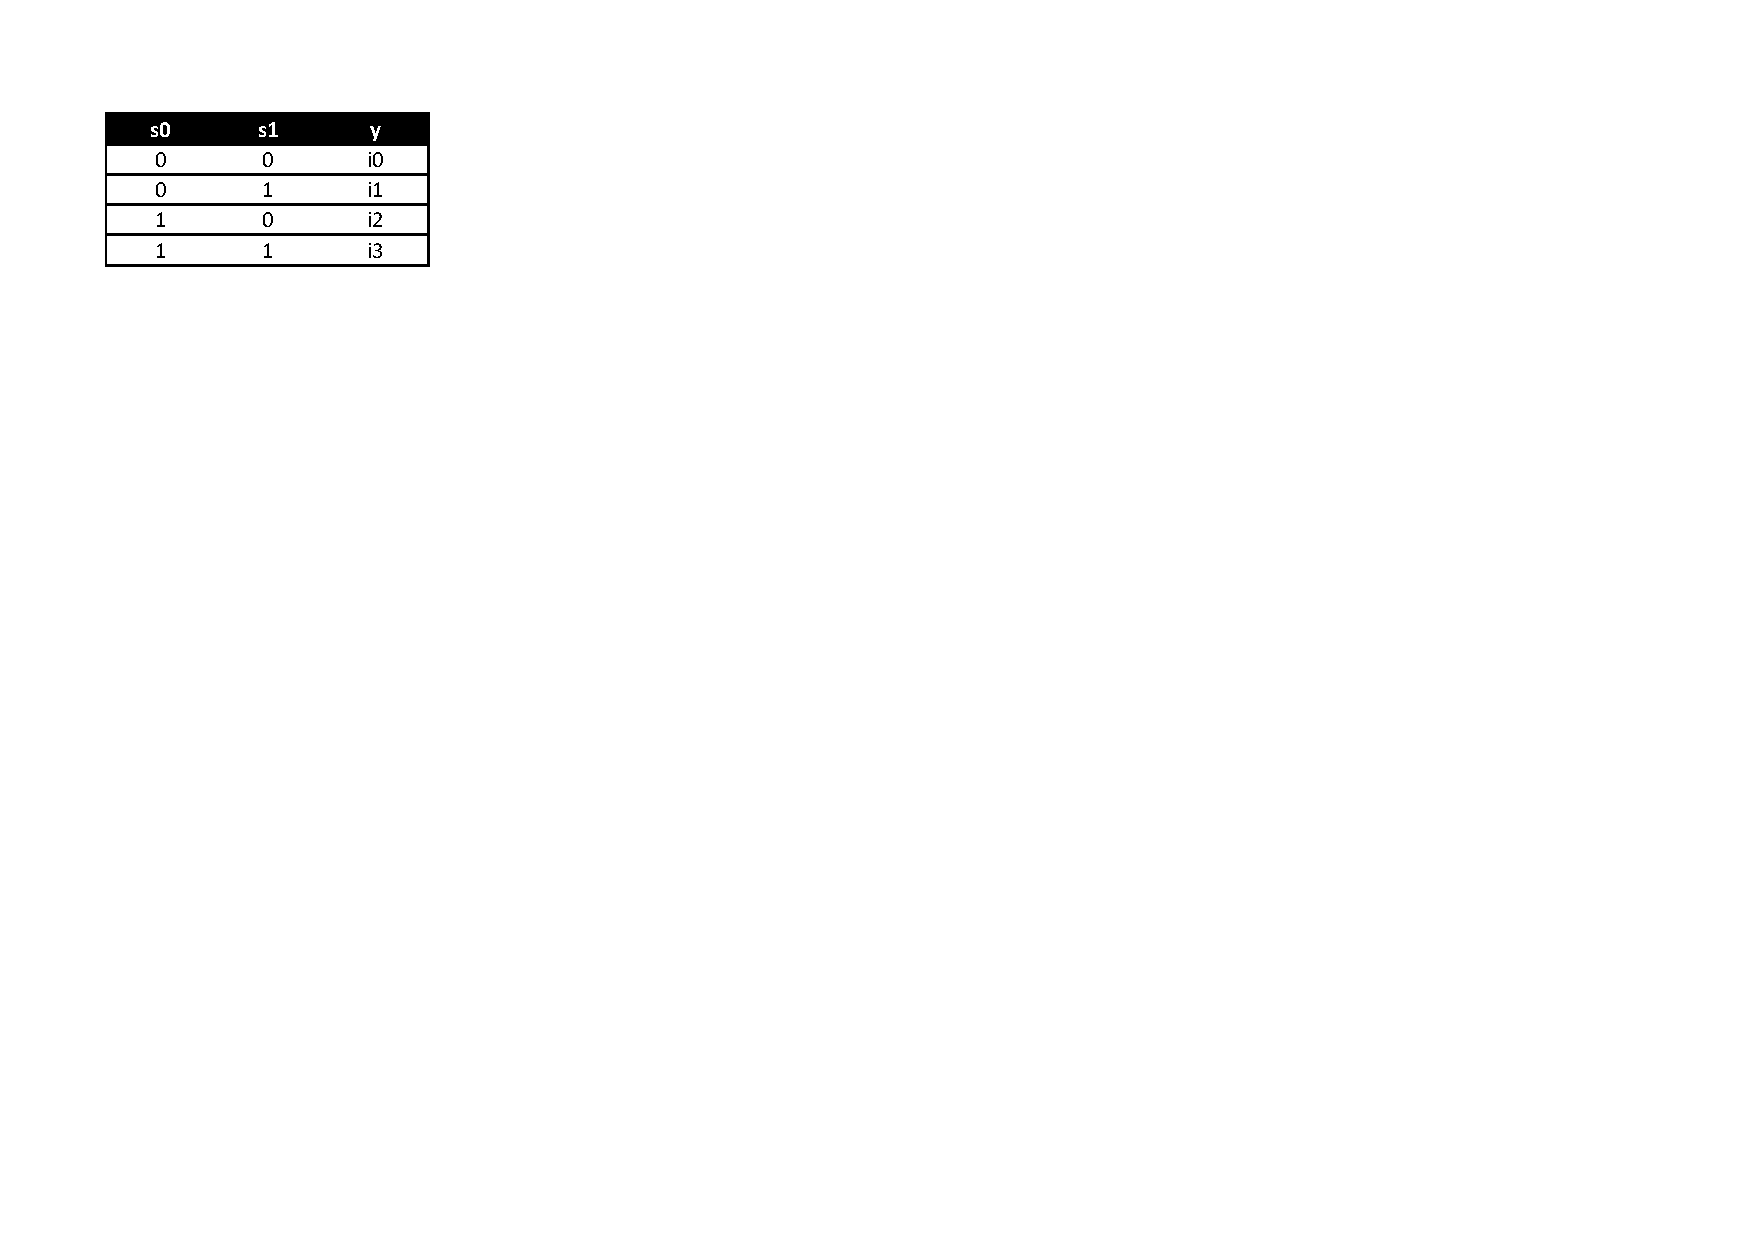
\includegraphics{tableMultiplexer}
	\caption{Truth table of 4$\times$1 multiplexer}
	\label{tbl:Multiplexer}
\end{table}


\subsection{Conditional signal assignment}

Syntax for conditional signal assignment is shown in lines 15-18 of Listing \ref{vhdl:multiplexerEx}, where `when' and `else' keywords are used for assigning the value to output port `y'. Conditional signal assignments are implemented using `2$\times$1' multiplexer as shown in Fig. \ref{fig:multiplexerEx}. Here, three `2$\times$1' multiplexer (i.e. y$\sim$0, y$\sim$2 and y$\sim$4) are used to design the `4$\times$1' multiplexer.

\lstinputlisting[
language = Vhdl,
caption    = {Multiplexer using Conditional signal assignment},
label      = {vhdl:multiplexerEx}
]{multiplexerEx.vhd}


\begin{figure}[!h]
	\centering
	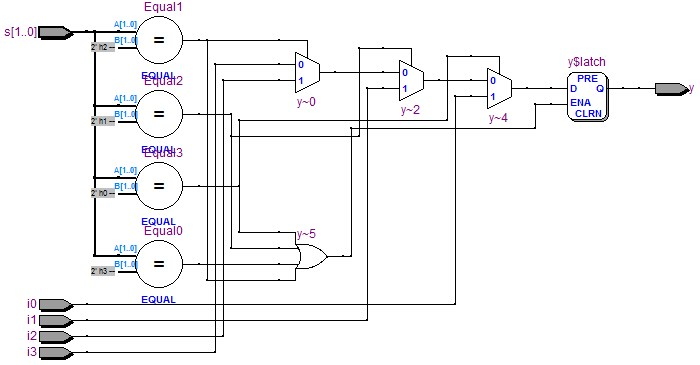
\includegraphics[width=0.8\textwidth]{multiplexerEx}
	\caption{Multiplexer using Conditional signal assignment}
	\label{fig:multiplexerEx}
\end{figure}

Fig. \ref{fig:multiplexerExWave} shows the waveform of Listing \ref{vhdl:multiplexerEx}. Here i0, i1, i2 and i3 are set to 1, 0, 1 and 0 respectively. Then simulator is run 4 times for all the combination of `s' i.e. 00, 01, 10 and 11 respectively; and output `y' is assigned the value based on the `s' value e.g if s is `00' then y is assigned with the value of `i0' i.e. 1 etc.  

\begin{figure}[!h]
	\centering
	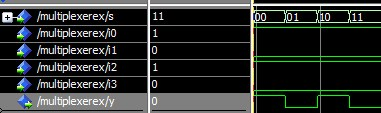
\includegraphics[scale=0.8]{multiplexerExWave}
	\caption{Multiplexer waveform for Listing \ref{vhdl:multiplexerEx} and \ref{vhdl:multiplexerVhdl}}
	\label{fig:multiplexerExWave}
\end{figure}



\subsection{Selected signal assignment}
Syntax for selected signal assignment is shown in lines 15-23 of Listing \ref{vhdl:multiplexerVhdl}, where `with-select' and `when' keywords are used for assigning the value to output port `y'. Unlike conditional signal statement, in selected signal assignment implements the 4$\times$1 multiplexer with 4$\times$1 multiplexer itself as shown in Fig. \ref{fig:multiplexerVhdl}, rather than with multiple 2$\times$1 multiplexer. Further, the waveforms for Listing \ref{vhdl:multiplexerVhdl} is shown in Fig. \ref{fig:multiplexerExWave}.

Note that `unaffected when others' is used in line 23.  `others' is used to avoid the error which is caused by the logics which can not be synthesized,  as mentioned in comments in lines 20-22. Further, `unaffected' is the keyword which does not allow any change in the signal.

\begin{figure}[!h]
	\centering
	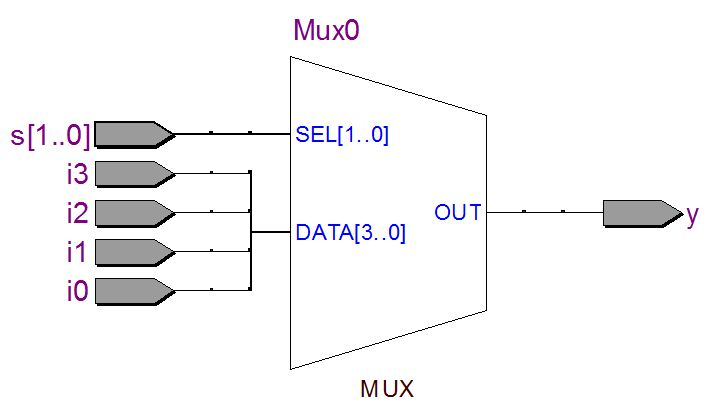
\includegraphics[scale=0.4]{multiplexerVhdl}
	\caption{Multiplexer using Selected signal assignment}
	\label{fig:multiplexerVhdl}
\end{figure}

\lstinputlisting[
language = Vhdl,
caption    = {Multiplexer using Selected signal assignment},
label      = {vhdl:multiplexerVhdl}
]{multiplexerVhdl.vhd}

\section{Generate statement and problem with Loops}

`Generate statement' is used for creating loops in concurrent assignments. These loops are very different from software loops. Suppose `for i = 1 to N' is a loop, then, in software `i' will be assigned one value at a time i.e. first i=1, then next cycle i=2 and so on. Whereas in VHDL, N logic will be implement for this loop, which will execute in parallel. Also, in software, `N' cycles are required to complete the loop, whereas in VHDL the loop will execute in one cycle. 
\begin{noNumBox}
	As loops implement the design-units multiple times, therefore design may become large and sometimes can not be synthesized as well. If we do not want to execute everything in one cycle (which is almost always the case), then loops can be replaced by `case' statements and `conditional' statements as shown in section \ref{sec:ifLoop}. Further, due to these reasons, we do not use loops in the design, and hence these are not discussed in the tutorial.
\end{noNumBox}   

\section{Conclusion}
In this chapter, we saw various features of Dataflow modeling style. We discussed the delays in VHDL designs. Also, 4$\times$1 multiplexer is implemented using conditional and selected signal assignments. Further, the differences in the designs generated by these two assignments are shown using figures.